\documentclass{article}

\usepackage{fullpage}

\usepackage{amsmath}
\usepackage{amssymb}
\usepackage{graphicx}
\usepackage[colorlinks,linkcolor=dblue,filecolor=black,citecolor=dblue,urlcolor=dblue]{hyperref}
\usepackage{etex}
\bibliographystyle{alpha}
\usepackage[english]{babel}
\usepackage{amsfonts,amssymb,amsmath,sectsty,url}
\usepackage{mathrsfs}
\usepackage{float}
\usepackage{tikz}
\usetikzlibrary{calc}
\usepackage{color}
%\usepackage{mathtools}
\usepackage[all]{xy}
\usepackage{ctable}
% \usetikzlibrary{calc}

\usepackage{graphicx}
\usepackage{ifpdf}
\usepackage{multirow}
\usepackage{multicol,color}
\usepackage{tablefootnote}


\usepackage{amsthm}
\usepackage{amsmath}


\theoremstyle{plain}
\newtheorem{theorem}{Theorem}[section]
\newtheorem{corollary}[theorem]{Corollary}
\newtheorem{lemma}[theorem]{Lemma}%[section]
\newtheorem{proposition}[theorem]{Proposition}%[section]

\theoremstyle{definition}
\newtheorem{definition}[theorem]{Definition}
\newtheorem{example}[theorem]{Example}%[section]
\newtheorem{construction}[theorem]{Construction}


\theoremstyle{remark}
\newtheorem{remark}[theorem]{Remark}
\newtheorem{fact}[theorem]{Fact}%[section]
\newtheorem{observation}[theorem]{Observation}
\newtheorem{claim}[theorem]{Claim}%[section]

\usepackage{algorithm}
\usepackage[noend]{algpseudocode}

\makeatletter
\def\BState{\State\hskip-\ALG@thistlm}
\makeatother


% COMMANDS

\renewcommand{\emptyset}{\varnothing}

% Colors

\definecolor{dblue}{rgb}{0.00, 0.50, 0.90}
\definecolor{lblue}{rgb}{0.70, 0.80, 1.00}
\definecolor{lpink}{rgb}{0.90, 0.70, 1.00}
\definecolor{lgreen}{rgb}{0.80, 0.95, 0.75}
\definecolor{lred}{rgb}{0.99, 0.50, 0.55}
\definecolor{lyellow}{rgb}{1.00, 0.95, 0.75}
\definecolor{llgrey}{rgb}{0.95, 0.95, 0.95}
\definecolor{salmon}{rgb}{0.99, 0.90, 0.90}

% UC security things

\newcommand{\secs}{\mathsf{aggregation}}
\newcommand{\Pss}{\Pi_\secs}
\newcommand{\Fss}{\mathcal F_\secs}
\newcommand{\Sss}{\mathcal S_\secs}


\newcommand{\elect}{\mathsf{election}}
\newcommand{\Pelect}{\Pi_\elect}
\newcommand{\Felect}{\mathcal F_\elect}
\newcommand{\Select}{\mathcal S_\elect}

\newcommand{\Commit}{\mathsf{Commit}}
\newcommand{\Open}{\mathsf{Open}}
\newcommand{\Pcomm}{\Pi_\Commit}
\newcommand{\Fcomm}{\mathcal F_\Commit}
\newcommand{\Scomm}{\mathcal S_\Commit}

\newcommand{\Fnoisegen}{\mathcal{F}_{\mathsf{noise}}}
\newcommand{\Pdpa}{\Pi_{\mathsf{dp}\textrm{-}\mathsf{aggregation}}}
\newcommand{\Pbinomial}{\Pi_\mathsf{binomial}}
\newcommand{\Pgauss}{\Pi_\mathsf{gauss}}
\newcommand{\Pfirstlaplace}{\Pi_\mathsf{laplace1}}
\newcommand{\Psecondlaplace}{\Pi_\mathsf{laplace2}}
\newcommand{\Ppack}{\Pi_\mathsf{pack}}


% CS things
\newcommand{\Oh}{ \mathcal{O} }
\newcommand{\QuasiOh}{ \widetilde{ \mathcal{O} } }

%\newcommand{\B}			{\mathrm{B}}
\newcommand{\KB}		{\mathrm{KB}}
\newcommand{\MB}		{\mathrm{MB}}
\newcommand{\GB}		{\mathrm{GB}}

\newcommand{\ms}		{\mathrm{ms}}
\newcommand{\mus}		{\mathrm{{\mu}s}}

% FE
\newcommand{\FE}{\mathsf{FE}} % FE
\renewcommand{\sec}{\lambda} % sec param
\newcommand{\PP}{\mathsf{PP}} % public parameters for FE
\newcommand{\MK}{\mathsf{MK}} % master secret key for FE
\newcommand{\Key}{\mathsf{Key}} % enc/dec secret key for (secret-key) FE
\newcommand{\Ctxt}{\mathsf{Ctxt}} % enc/dec secret key for (secret-key) FE

\renewcommand{\sf}{\mathsf{sf}} % semi-functional flag
\newcommand{\f}{\mathsf{f}} % functional flag


% Encodings
\newcommand{\A}{\mathbf{A}} % matrix for encoding
\renewcommand{\S}{\mathbf{S}} % secret matrix (tensored)
\newcommand{\B}{\mathbf{B}} % BP matrix
\newcommand{\E}{\mathbf{E}} % error matrix
\newcommand{\Y}{\mathbf{Y}} % result encoding matrix
\newcommand{\D}{\mathbf{D}} % trapdoor'd matrix
\newcommand{\J}{\mathbf{J}} % left bookend

\newcommand{\TrapSam}{\mathsf{TrapSam}}
\newcommand{\PreimgSam}{\mathsf{PreimgSam}}



% Sets, fields, rings, groups, etc...
\newcommand{\Id}{\mathbb{I}} % the identity matrix
\newcommand{\Z}{\mathbb{Z}} % the integers
\newcommand{\N}{\mathbb{N}} % the non-negative integers
\newcommand{\F}{\mathbb{F}} % a finite field
\newcommand{\K}{\mathbb{K}} % a finite field
\newcommand{\Kbot}{\mathbb{K}_{\bot}} % a finite field extended with bottom

\renewcommand{\P}{\{1,\dots,n\}} % player set $\{1,\dots,n\}$

%\newcommand{\K}{\mathcal{K}} % key space
\newcommand{\M}{\mathcal{M}} % message space
\newcommand{\T}{\mathcal{T}} % tag space
\newcommand{\R}{\mathcal{R}} % randomness space

\newcommand{\tensor}{\otimes}
\newcommand{\unit}{\mathbf{u}}
\newcommand{\transpose}[1]{#1^{\intercal}}
\newcommand{\identitymatrix}{\mathbb{I}}
%\newcommand{\identitymatrix}{\mathbb{1}}  % requires the bbold package
%\newcommand{\cartesian}[1]{{\times #1}}
\newcommand{\cartesian}[1]{{\times \! #1}}
%\newcommand{\cprod}{\bigtimes}  % requires the mathabx package



% Probability and DP
\newcommand{\Avg}{\textup{E}} % Average of random variables

\newcommand{\mechanism}[1]{\mathcal{ #1 }}
\newcommand{\norm}[1]				{\left\lVert #1 \right\rVert}
\newcommand{\e}	[1]						{\mathbf{e}^{#1}}
%\newcommand{\e}	[1]						{\mathrm{exp}(#1)}
\newcommand{\sensitivity}[2]		{\Delta_{#1} #2}
\newcommand{\intype}					{\mathcal{X}}
\newcommand{\dstype}					{\N^{\intype}}
\newcommand{\ds}						{D}

\newcommand{\given}			{\; | \;}
\newcommand{\condpr}[2]		{\pr{#1 \given #2}}
\newcommand{\distsOver}[1]		{\Delta #1}

%\newcommand{\hammingweight}[1]	{\mathrm{H}(#1)}
\newcommand{\hammingweight}[1]	{\mathrm{w_H}(#1)}

%\newcommand{\D}{\mathcal{D}} % a distribution
\newcommand{\U}{\mathcal{U}} % the uniform distribution

\newcommand{\coin}						{\mathcal{C}}
\newcommand{\uniform}[1]			{\mathcal{U}(#1)}
\newcommand{\binomial}[1]			{\mathcal{B}(#1)}
\newcommand{\gaussian}[1]			{\mathcal{N}(#1)}
\newcommand{\laplacian}[1]			{\mathrm{Lap}(#1)}
\newcommand{\distribution}			{\mathcal{D}}
\newcommand{\leftovernoise}		{\mathcal{E}}

\newcommand{\pr}[1]					{\Pr \left[ #1 \right]}
\newcommand{\floor}[1]					{\lfloor#1\rfloor}
\newcommand{\ceil}[1]					{\left\lceil#1\right\rceil}



% Labels

\newcommand{\pk}{\mathsf{pk}}
\newcommand{\sk}{\mathsf{sk}}


\newcommand{\off}{\texttt{off}}

\newcommand{\Sim}{\mathcal{S}}



% Operators

\newcommand{\AND}{\wedge}
\newcommand{\OR}{\vee}
\newcommand{\bigAND}{\bigwedge}
\newcommand{\bigOR}{\bigvee}

\newcommand{\asn}{\gets} % to be read as ``computed as'' or ``taken according to the distribution...'' or ``taken uniformly from...''

\newcommand{\ParamGen}{\mathsf{ParamGen}}
\newcommand{\Setup}{\mathsf{Setup}}
\newcommand{\KeyGen}{\mathsf{KeyGen}}
\newcommand{\Enc}{\mathsf{Enc}}
\newcommand{\Dec}{\mathsf{Dec}}
\newcommand{\Add}{\mathsf{Add}}
\newcommand{\ek}{ek}
\newcommand{\dk}{dk}
\newcommand{\plaintext}{m}
\newcommand{\ciphertext}{e}
\newcommand{\plaintextspace}{\mathcal{P}}
\newcommand{\ciphertextspace}{\mathcal{E}}
\newcommand{\INDCPA}{\textrm{IND-CPA}}

\newcommand{\Share}{\mathsf{Share}}
\newcommand{\SimShare}{\mathsf{SimShare}}
\newcommand{\Shamir}{\mathsf{Shamir}}
\newcommand{\PackedShamir}{\mathsf{PackedShamir}}
\newcommand{\RS}{\mathsf{RS}}
\newcommand{\Rec}{\mathsf{Recon}}
\newcommand{\SSS}{\mathsf{SSS}}

\newcommand{\share}{\sigma}
\newcommand{\secret}{m}

\newcommand{\MAC}{\mathsf{MAC}}
\newcommand{\Encode}{\mathsf{Encode}}


\newcommand{\Adv}{\mathsf{Adv}}
\newcommand{\Gen}{\mathsf{Gen}}
\newcommand{\AExpm}{\mathsf{Exp}}



\newcommand{\ineff}{\mathsf{ineff}}
\newcommand{\superpoly}{\mathsf{superpoly}}
\newcommand{\poly}{\mathsf{poly}}
\newcommand{\negl}{\mathsf{negl}}
\newcommand{\const}{\mathsf{const}}
\newcommand{\polylog}{\mathsf{polylog}}

\newcommand{\normtwo}[1]{\|{#1}\|_2}
\newcommand{\normI}[1]{\|{#1}\|_\infty}



% Environments
\newenvironment{boxfig}[2]{% {#1}{#2} = {Caption}{label}
\begin{figure}[ht!]
  \newcommand{\FigCaption}{#1}
  \newcommand{\FigLabel}{#2}
  \vspace{-\medskipamount}
  \begin{center}
    \begin{small}
      \begin{tabular}{@{}|@{~~}l@{~~}|@{}}
        \hline
        \rule[-1.5ex]{0pt}{1ex}
        \begin{minipage}[b]{.96\linewidth}
          \vspace{1ex}
          \smallskip
          }{%
        \end{minipage}\\
        \hline
      \end{tabular}
    \end{small}
    \vspace{-1\bigskipamount}
  \end{center}
    \caption{\small \FigCaption}
    \label{\FigLabel}
%  \vspace{-0.3cm}
\end{figure}
}



% LATEX

% this crossreferences description items
\makeatletter
\let\orgdescriptionlabel\descriptionlabel
\renewcommand*{\descriptionlabel}[1]{%
  \let\orglabel\label
  \let\label\@gobble
  \phantomsection
  \edef\@currentlabel{#1}%
  %\edef\@currentlabelname{#1}%
  \let\label\orglabel
  \orgdescriptionlabel{#1}%
}
\makeatother




% a temporary counter
\newcounter{tempcount}


\newcommand{\mr}[1]{{\textcolor{lblue}{\textbf{Mariana:} #1}}}
\newcommand{\vc}[1]{{\textcolor{lred}{\textbf{Valerie:} #1}}}
\newcommand{\vp}[1]{{\textcolor{dblue}{\textbf{Valerio:} #1}}}

\title{Multiparty Linear Regression via SPDZ}
\author{Valerie Chen \and Valerio Pastro \and Mariana Raykova}
\date{}

\begin{document}

\maketitle

\section{Background}

Regression analysis and other machine learning techniques aim to build a model that fits a set of predictors to the dependent variable. These are commonly utilized technique in real world industries ranging from finance to medicine to security and can be crucial in understanding large scale consumer behavior. With the advent of big data and recent technological advances, it is becoming increasingly simple for entities to store vast amounts of user data. For example, individual hospitals might have their own patient data, but sharing this data for prediction or model-building purposes would be against modern day privacy laws. Secure multi-party computation (MPC) aims to solve this problem by providing a mechanism through which different parties and supply their data for joint computation without revealing individual values in each database.\\

\noindent
Two common regression techniques are linear and logistic regression. These are the fundamental building blocks for many more complex machine learning algorithms. In this project, our goal was to evaluate the efficacy of SPDZ as a viable secure multi-party framework for complex regression and machine learning algorithms. This paper also briefly explores the efficacy of neural networks in a secure computation setting.\\

\noindent
Insert stuff about SPDZ background / why we chose to use it over other things. \\ 

\noindent
Two previous works that this paper specifically builds off of are [1,2]. 

\section{Algorithms}

Our goal was to conduct a thorough investigation of the SPDZ framework in comparison to other similar frameworks of similar nature [1,2]. The main algorithms that we considered were, LDLT Decomposition, Cholesky, Conjugate Gradient Descent (CGD), Stochastic Gradient Descent (SGD), Logistic Regression, and Neural Networks. The algorithms for the first three were first presented in [1] and the latter two in [2], but in the sections below we further detail the algorithms and modifications that were made to them to accomodate the SPDZ framework. The algorithms were implemented in the SPDZ framework as a proof-of-concept as well as in python as a plaintext verification of the accuracy of the secure version. Even though the files that is inputted into SPDZ are almost derived from python, there were capabilities that were missing in this framework that directly impacted the implementation of the algorithm. The following subsections detail the five algorithms that were investigated in this work as well as SPDZ specific changes that were made to make the implementation work. \\

\noindent
A general problem that differed SPDZ from a numpy framework in python was the lack of  vectorization, meaning there was no support for matrix operations. This made sense because even basic arithmetic and multiplication was difficult to implement in a secure setting. However, we see this as an important avenue of development due to the increasing importance of ... finish this sentence. LOOK INTO HOW MATRICES ARE WRITTEN - are there operations?

\subsection{Cholesky}

The Cholesky decomposition algorithm relies on having a Hermitian positive-definite matrix A and a vector b as input and outputs a factorization of the form $LL^T$ where $L$ is a lower triangular matrix with real and positive diagonal entries and $L^T$ is the conjugate transport of L, which in this case is just $L^T$. Then using $L$, we compute $y$ where $L^Ty = b$. Finally the solution $\beta$ where $A\beta = y$ is computed. When given a matrix that fits the Hermitian, positive-definite pattern, this method outperforms traditional LU decomposition, for solving linear equations. A more detailed algorithm is presented below: 

\begin{algorithm}[H]
\caption{}\label{euclid}
\begin{algorithmic}[1]
\State $\textit{Let a be the input matrix, d be dimensions}$
\State 1. Decompose into $LD$
\For {j = 0, $j < d$}
\For {k = 0, $k < j$}
\For {i = j, $i < d$}
\State $a[i][j] = a[i][j] - (a[i][k] *a[j][k])$.
\EndFor
\State $a[j][j] = sqrt(a[j][j])$
\For {k = j+1, k < d}
\State $a[k][j] = a[k][j] / a[j][j]$
\EndFor 
\EndFor
\EndFor
\State 2. Compute $y$ where $L^Ty = b$
\For {i = 0, $i < d$}
\For {j = 0, $j < i$}
\State $b[i] = b[i] - (a[i][j] * y[i])$
\EndFor 
\State $y[i] = b[i] / a[i][i]$
\EndFor
\State 3. Compute the solution $\beta$ where $A\beta = y$
\For {$i = d-1$, $i \geq 0$, $i = i - 1$}
\For {j = 0, $j < i$}
\State $b[i] = b[i] - (a[i][j] * y[i])$
\EndFor 
\State $y[i] = b[i] / a[i][i]$
\EndFor
\end{algorithmic}
\end{algorithm}
Runtime

\subsection{LDLT}

The $LDL^T$, also known as the LDL decomposition, algorithm is a close variant of the Cholesky algorithm presented in the section above. As the name suggests, the input matrix A is factored into $LDL^T$, where $L$ is a lower triangular matrix and $D$ is a diagonal matrix. We can then use $L$ and $D$ to solve for the solution to the linear equations by computing $b'$ where $Lb' = b$ and then the solution $b''$ where $Db'' = b'$. A detailed algorithm is detailed below: 

\begin{algorithm}[H]
\caption{}\label{euclid}
\begin{algorithmic}[1]
\State $\textit{Let a be the input matrix, d be dimensions, b be the output vector}$
\State 1. Decompose into $LD$
\For {j = 0, $j < d$}
\For {k = 0, $k < j$}
\State $temp = a[j][k] * a[k][k]$
\For {i = j, $i < d$}
\State $a[i][j] = a[i][j] - (a[i][k] *temp)$.
\EndFor
\For {k = j+1, k < d}
\State $a[k][j] = a[k][j] / a[j][j]$
\EndFor 
\EndFor
\EndFor
\State 2. Compute $b'$ where $Lb'= b$
\For {i = 0, $i < d$}
\For {j = 0, $j < i$}
\State $b[i] = b[i] - (a[i][j] * b[j])$
\EndFor 
\EndFor
\State 3. Compute $b''$ where $Db'' = b'$
\For {i = 0, i < d}
\State $b[i] = b[i] / a[i][i]$
\EndFor 
\State 4. Compute $\beta$ where $L\beta = b''$ 
\For {$i = d-1$, $i \geq 0$, $i = i - 1$}
\For {$j = d-1$, $j > i$, $j = j -1$}
\State $b[i] = b[i] - (a[j][i] * b[j])$
\EndFor 
\EndFor
\end{algorithmic}
\end{algorithm}

\noindent
Runtime. The LDL variant, if efficiently implemented, requires the same space and computational complexity to construct and use but avoids extracting square roots. 

\subsection{Conjugate Gradient Descent}

Conjugate Gradient Descent, also known as CGD, is a popular numerical method for solving linear equations of the symmetric, positive-definite form. The difference between CGD and the previous two algorithms is that this is iterative, which makes it particularly suitable for large systems where a direct decomposition method would be too slow. 

\begin{algorithm}[H]
\caption{}\label{euclid}
\begin{algorithmic}[1]
\State $\textit{Let a be the input matrix, d be dimensions}$
\State $\theta = [0]*n$
\State $gtilda = [0]*n$
\State $p = [0]*n$
for

\For {$i = 0$, $i < iterations$}
\EndFor
\end{algorithmic}
\end{algorithm}

Look at paper for algorithm modifications.

Runtime why iterative makes it better

\subsection{Stochastic Gradient Descent}

Stochastic Gradient Descent, or SGD, \\

\noindent
Talk about batch normalization, which is also applicable to logistic regression.

\begin{algorithm}[H]
\caption{}\label{euclid}
\begin{algorithmic}[1]
\Procedure{MyProcedure}{}
\State $\textit{stringlen} \gets \text{length of }\textit{string}$
\State $i \gets \textit{patlen}$
\BState \emph{top}:
\If {$i > \textit{stringlen}$} \Return false
\EndIf
\State $j \gets \textit{patlen}$
\BState \emph{loop}:
\If {$\textit{string}(i) = \textit{path}(j)$}
\State $j \gets j-1$.
\State $i \gets i-1$.
\State \textbf{goto} \emph{loop}.
\State \textbf{close};
\EndIf
\State $i \gets i+\max(\textit{delta}_1(\textit{string}(i)),\textit{delta}_2(j))$.
\State \textbf{goto} \emph{top}.
\EndProcedure
\end{algorithmic}
\end{algorithm}

\subsection{Logistic Regression}

Another popular regression method for two-class classification problems is logistic regression. The update function is a modification of the SGD update, $ w = w - \frac{1}{|B|} \alpha X^{T}_{B} \times (f(X_{B} \times w) - Y_{B})$ where $f(u)$ is the activation function $\frac{1}{1+e^{-u}}$. However, the exponential function is difficult to achieve in a secure setting, so one alternative is to approximate an exponential using a Taylor series and another is to use the secure computation friendly activation piecewise function defined by [2]: 

\[
  f(u) =
  \begin{cases}
                                   0 & \text{if $u < -0.5$} \\
                                   u + 0.5 & \text{if $-0.5 \leq u \leq 0.5$} \\
1 & \text{if $u > 0.5$}
  \end{cases}
\]


What distinguishes logistic regression from the previous linear regression algorithms is the use of a nonlinear activation function. 

\begin{algorithm}[H]
\caption{}\label{euclid}
\begin{algorithmic}[1]
\Procedure{MyProcedure}{}
\State $\textit{stringlen} \gets \text{length of }\textit{string}$
\State $i \gets \textit{patlen}$
\BState \emph{top}:
\If {$i > \textit{stringlen}$} \Return false
\EndIf
\State $j \gets \textit{patlen}$
\BState \emph{loop}:
\If {$\textit{string}(i) = \textit{path}(j)$}
\State $j \gets j-1$.
\State $i \gets i-1$.
\State \textbf{goto} \emph{loop}.
\State \textbf{close};
\EndIf
\State $i \gets i+\max(\textit{delta}_1(\textit{string}(i)),\textit{delta}_2(j))$.
\State \textbf{goto} \emph{top}.
\EndProcedure
\end{algorithmic}
\end{algorithm}

Another challenge to implementing logistic regression is that SPDZ does not support branching using if statements, since comparing a secret value without revealing the internal value will always return, no matter the comparison on the actual value. To work around this, we need to convert the piecewise function into circuits.

\subsection{Neural Networks}

Neural networks are extensions of the more basic regression algorithms presented above, which includes multiple layers of neurons and forward and backpropagation through the layers. Per the experiments in [2], we used two hidden layers and 128 neurons per layer.

After each layer is a nonlinear activation function and an area worth experimenting in terms of MPC is the best type of activation function, which includes 

We experiment with both the RELU and the square function as the activation function in the hidden layers and our proposed alternative to softmax function in the output layer. 

Write out the formulas... as well as detail the implementation of approximating the activation function as well as softmax. 

Since [2] did not detail the protocol, we provide a more in-depth description for replicating our results. 

\begin{algorithm}[H]
\caption{}\label{euclid}
\begin{algorithmic}[1]
\Procedure{MyProcedure}{}
\State $\textit{stringlen} \gets \text{length of }\textit{string}$
\State $i \gets \textit{patlen}$
\BState \emph{top}:
\If {$i > \textit{stringlen}$} \Return false
\EndIf
\State $j \gets \textit{patlen}$
\BState \emph{loop}:
\If {$\textit{string}(i) = \textit{path}(j)$}
\State $j \gets j-1$.
\State $i \gets i-1$.
\State \textbf{goto} \emph{loop}.
\State \textbf{close};
\EndIf
\State $i \gets i+\max(\textit{delta}_1(\textit{string}(i)),\textit{delta}_2(j))$.
\State \textbf{goto} \emph{top}.
\EndProcedure
\end{algorithmic}
\end{algorithm}

\section{Datasets}

This paper used a combination of existing, well-known and synthetically generated data. Many other papers (give examples) have also explored the MNIST and Arcene datasets as the canonical dataset for a proof-of-concept model. The MNIST is a classification dataset which consists of 60,000 black and white images of handwritten numbers from 0 to 9 scaled to a 28x28 pixel size. Each pixel is used as a feature which gives 784 total features in the dataset. The Arcene dataset is a two-class classification problem to distinguish cancerous from normal patients through mass spectrometric data. The mass spectrometric data is highly dimensional, with 10,000 features. A clarification of [2] is that we only explore both datasets in a binary setting, which is why the accuracy is so high for MNIST in particular.\\

\noindent
[1] presented a method for synthetic data generation that allowed varying of a few parameters which we took advantage to test the linear regression algorithms in different settings. The algorithm automatically 

Talk about condition numbers here... ?

\section{Experiments} 

The experiments for each algorithm were run in the SPDZ framework. The data that we ran our experiments on were a combination of synthetic and real data sets. For each data set, the features were split evenly between two parties. The main points of consideration when running the algorithms was the precision of the results as well as the total runtime in the secure setting. \\

\noindent
Typically both parties were run on one machine but we also performed tests where both parties were deployed on different Amazon EC2 instances. It is important to note that the distribution of players across machine only affects runtime and not the accuracy of the results. 

\subsection{Cholesky, LDLT, and CGD}

We primarily used a 128 bit and 256 bit prime field in SDPZ. In the 128 bit prime field, the bits were allotted with 28 bits after the decimal place to match the 32 bit example in the original paper and 60 bits after the decimal for the original 64 bit case. Compared to [1] we needed more space to the left of the decimal for to avoid overflow in operations using the fixed point type. However, this is still a fair comparison because we are not utilizing with more precision after the decimal place, and rather would actually increase run time.\\

\noindent
First, we ran the two algorithms two gauge time and error rates for synthetic matrices of size 10, 20, 50, 100, 200, and 500, with 10000 entries. As expected, utilizing more bits gives much better accuracy. In both cases, the error results are comparable to the garbled circuits paper. However, we found the original experiment truncated the generated data at 12 decimal places, however we modified it so that we could work with the full representation of the number. These are the average results over 30 samples with an average condition number of 1.77.

\begin{figure}[h]
\centering
  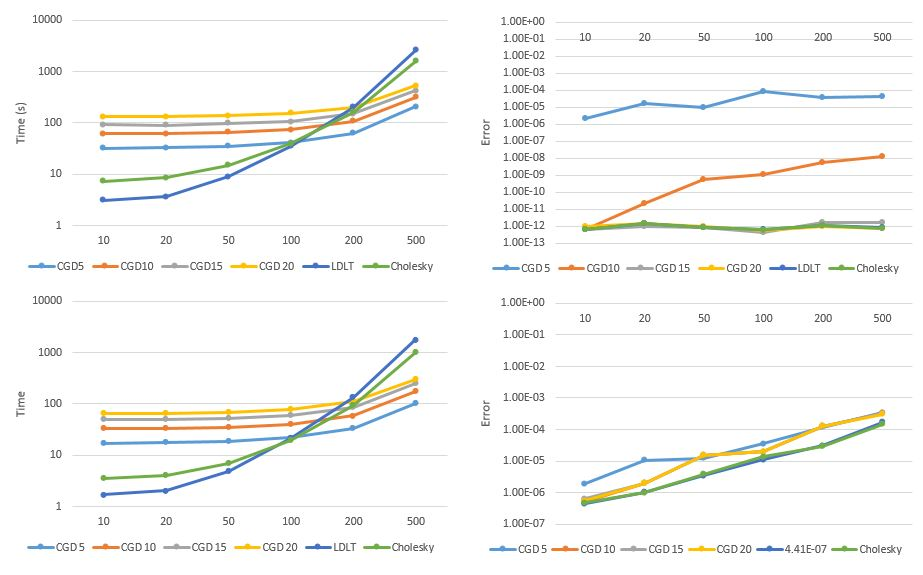
\includegraphics[scale=0.47]{results1.jpg}
  \caption{(Left) Run time comparison in seconds as a function of input dimension. (Right) Accuracy as a function of the input dimensionality $d$. (Top) Fixed-point numbers with the $b = 80$ bits, with 60 in the fractional part. (Bottom) $b = 41$, with 28 in the fractional part}
  \label{fig:result2}
\end{figure}

\noindent
We also varied the size of $N$ to see the effect of how different numbers of entries changed the accuracy of the algorithm. We noticed that the condition number of the matrix varies inversely with the amount of data in the system. More data means smaller condition number and thus better accuracy.

\begin{figure}[h]
\centering
  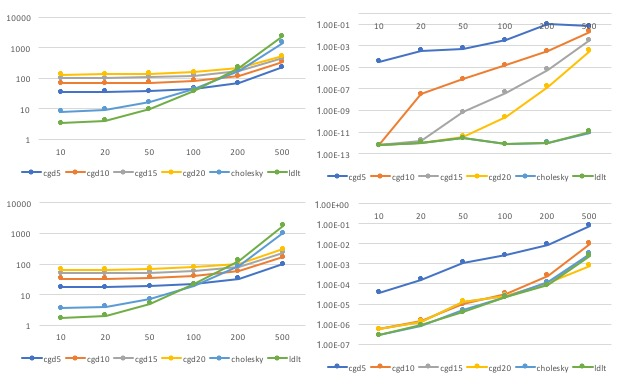
\includegraphics[scale=0.5]{results2.jpg}
  \caption{(Left) For N = 1000: Comparison between different methods of solving linear systems: running time in seconds for Cholesky, LDLT, and CGD as a function of input dimension. (Right) Accuracy of Cholesky, LDLT, and CGD, as a function of the input dimensionality $d$. (Top) Fixed-point numbers with the $b = 80$ bits, with 60 in the fractional part. (Bottom) $b = 41$, with 28 in the fractional part}
  \label{fig:result2}
\end{figure}  

\noindent
Secondly, we ran on a size 20 and size 100 matrices with varying condition numbers from 1 to 10. To replicate [1] we ran iterations of 5, 10, 15, and 20 for the CGD algorithm but also tried 25 iterations to see if there were improvements. 
\begin{figure}[H]
\centering
  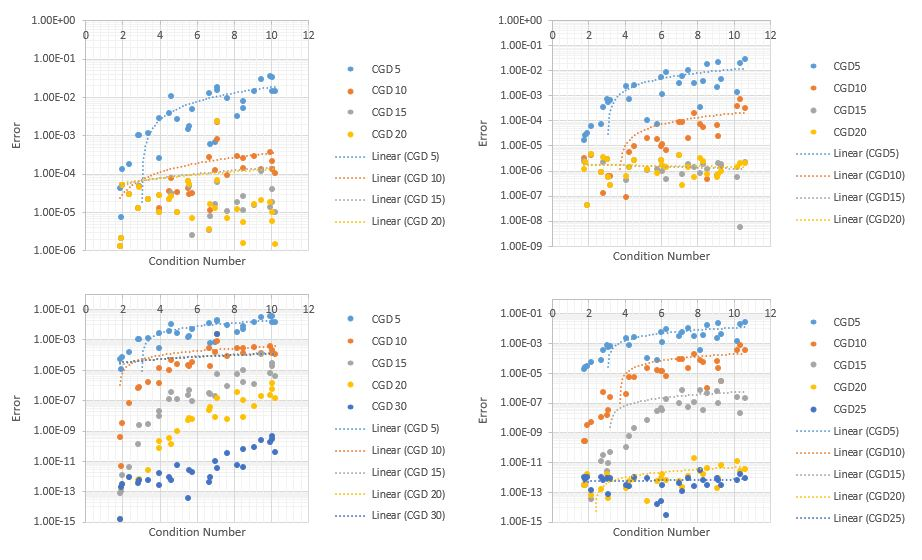
\includegraphics[scale=0.6]{conditionnumber.jpg}
  \caption{(Left) The plot of solving data with condition numbers ranging from 1 to 10 against the error, using matrices of size d = 100. (Right) The plot of solving data with condition numbers ranging from 1 to 10 against the error, using matrices of size d = 20. (Top) was ran in 32 bit SPDZ and (Bottom) was ran in 64 bit SPDZ.}
  \label{fig:result3}
\end{figure}

\noindent
In the condition number experiment, for CGD iterations of 5, 10, and 15, error increases as condition number increases. For example, in CGD 10 a small condition number may have an error of $\mathtt{10e-9}$ yet a larger condition number could have an error as large as $\mathtt{10e-3}$. However, in the CGD 20 case, the condition number does not have much effect due to the small errors, with the error varying only form $\mathtt{10e-11}$ to $\mathtt{10e-14}$. For the 60 bit precision case, we ran more iterations because there is a noticeable upward slope in the scatter plot in the CGD 20 line, indicating that still as condition numbers increased, the errors were increasing as well. Indeed, 25 iterations showed some improvement as we can see a flatter trend.\\

\noindent
To fine tune the CGD and Cholesky algorithms to SPDZ, we experimented with different ways of approximating square roots, to see if one or the other had better runtime or smaller error. The Babylonian method involves iteratively dividing and averaging an initial guess so on the next iteration can be represented as $x_{n+1} = \frac{1}{2} (x_{n} + \frac{S}{x_{n}})$. The Newton Method is similar but finds the square root using multiplications and not divisions: $\sqrt{S} = S \cdot (1/\sqrt{S})$. We originally hypothesized that using more multiplications over divisions should result in faster results. The results presented here are run on the Cholesky algorithm. However, since multiplication and division are implemented similarly in SPDZ, we did not find these results to be significant.

\begin{figure}[h]
     \centering
  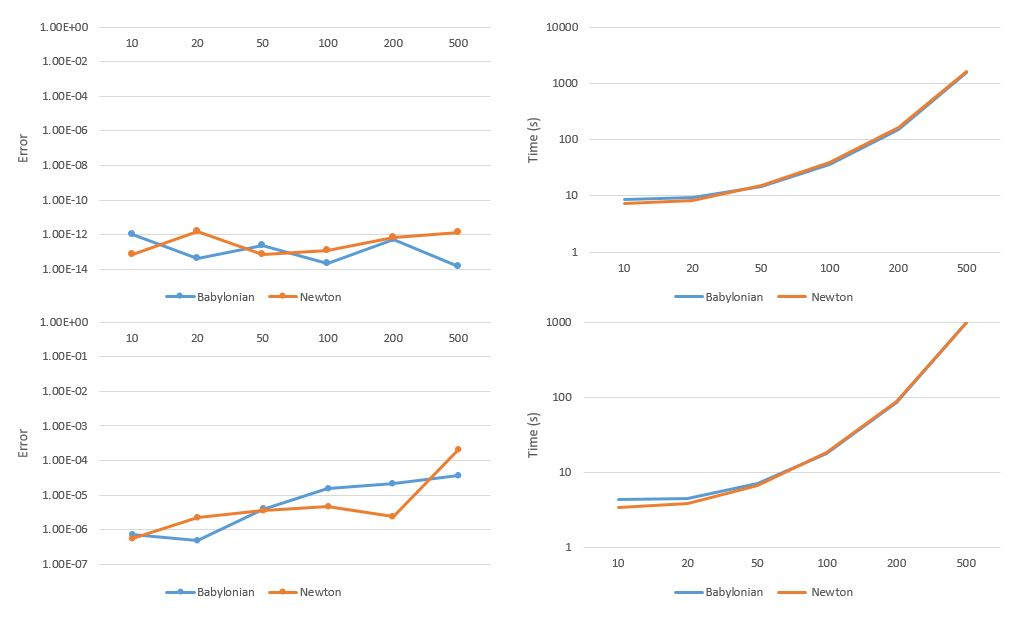
\includegraphics[scale=0.45]{sqrt.jpg}
  \caption{ 64 bit (top) and 32 bit (bottom) results for comparing approximating square roots methods.}
  \label{fig:result1}
\end{figure}

\noindent
For CGD, we decide to test if utilizing L2 norm vs Linfinity would make a difference in the algorithm. One utilizes comparisons which could be costly for arithmetic circuits and the other addition and square root. 

\begin{figure}[H]
\centering
  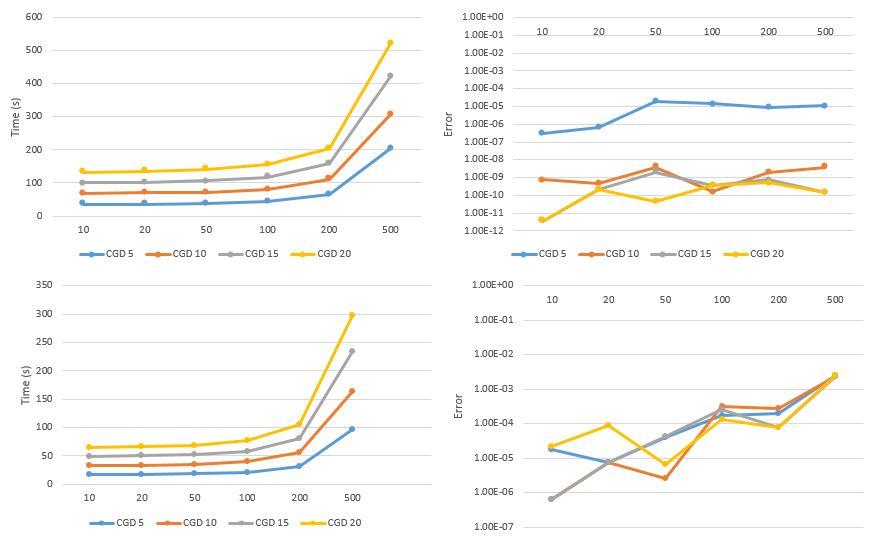
\includegraphics[scale=0.45]{l2.jpg}
  \caption{ (Top) 64 bit (Bottom) 32 bit results for L2 Norm. }
  \label{fig:result1}
\end{figure}

\subsection{Experiments on multiple parties and machines}

We also ran results for 3 and 4 players, which is also something that [1] considered. In a typical real world setting, there are often more than 2 parties, so we wanted to gauge what the additional run time would be for SPDZ to handle more parties. The error results were the same as those presented prior so we chose not to include them again. 

\begin{figure}[h]
\centering
  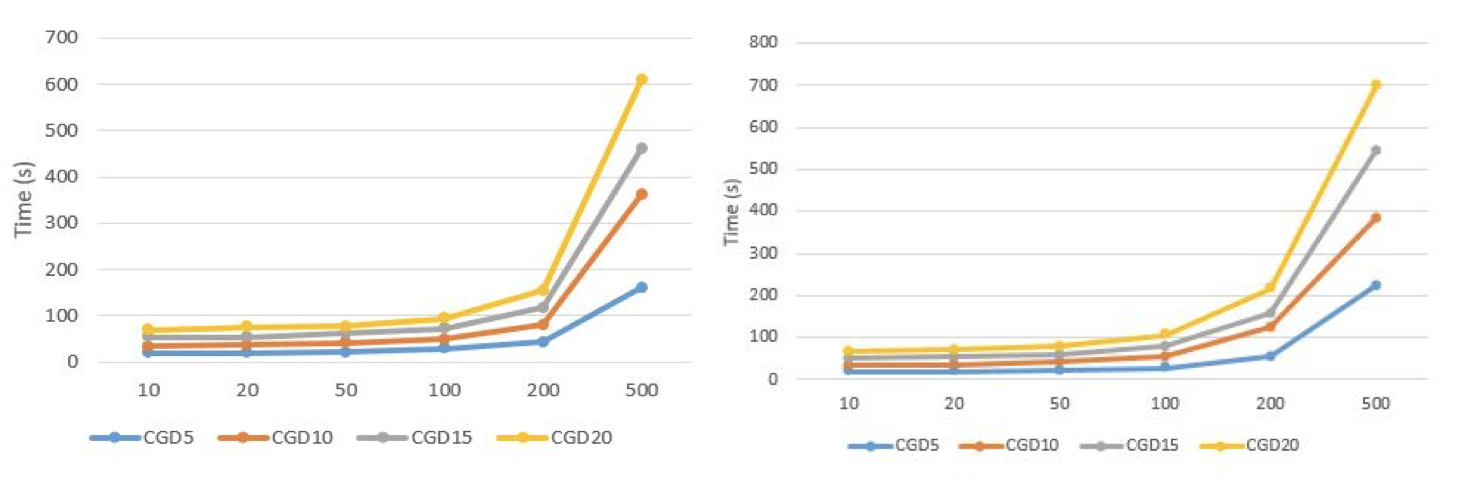
\includegraphics[scale=0.6]{multi.jpg}
  \caption{Run time results for 3 and 4 players in 32 bits. (Left) 3 Players. (Right) 4 Players.}
  \label{fig:result4}
\end{figure}

\noindent
Additionally, we deployed two Amazon EC2 instances of the c4.8xlarge type and performed the same experiments as before to gauge the latency of having two players on separate machines. The errors were the same as before, but we observed a drastic increase in run time over a network, compared to the previous two player results. 

\begin{figure}[h]
\centering
  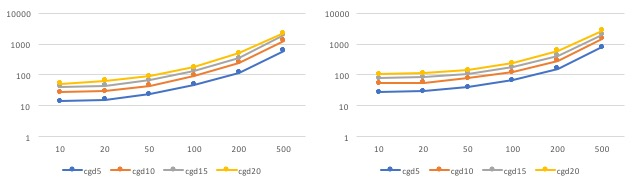
\includegraphics[scale=0.7]{ec2.jpg}
  \caption{Run time results for 2 players deployed on EC2 instances averaged over 15 runs. (Left) 32 bits. (Right) 64 bits.}
  \label{fig:result4}
\end{figure}

\subsection{Stochastic Gradient Descent}

To implement SGD, we utilized the update function presented in [2]: $ w = w - \frac{1}{|B|} \alpha X^{T}_{B} \times (X_{B} \times w - Y_{B})$. The first dataset that we worked with was MNIST, which contain 28 by 28 pixels of handwritten numbers and their corresponding labels. While the numbers in MNIST range from 0 to 9, [2] turned it into a binary problem by only using the handwritten 0 and 1s. The second dataset was Arcene which is also a two-class problem of cancer versus noncancerous spectrometric data. From Figure 8, we can observe that 13 bits are sufficient enough to achieve almost perfect accuracy for prediction.

\begin{figure}[H]
\centering
  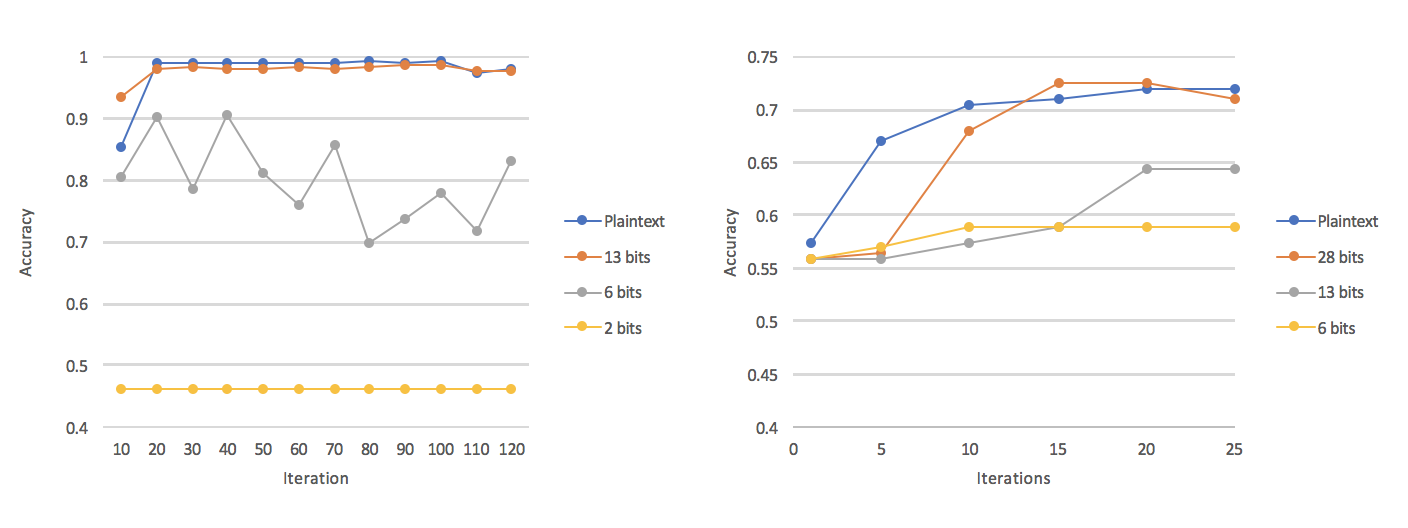
\includegraphics[scale=0.6]{mnistarcene.png}
  \caption{Varying number of bits and recreating results for MNIST (left) and Arcene (right) in [2].}
  \label{fig:result4}
\end{figure}

\noindent
The dimensions of the vector that we were predicting for MNIST was only 784, which comes from the 28 by 28 image. This is small compared to the size 10,000 vector that Arcene has. This could be an explanation for why the SGD prediction capabilities are not as good for Arcene when compared to MNIST and could explain why we need more bits in SPDZ to achieve plaintext comparable accuracy. 

\noindent
\\Using the same SGD algorithm, we also compared the resulting root mean squared error (RMSE) in 7 open sourced datasets of ranging sizes.

\begin{table}[H]
\centering
\label{my-label}
\begin{tabular}{@{}llllll@{}}
\toprule
Dataset Name          & \multicolumn{1}{c}{SGD Plaintext} & \multicolumn{2}{c}{\begin{tabular}[c]{@{}c@{}}SPDZ (28 bit)\\ error / time\end{tabular}} & \multicolumn{2}{c}{\begin{tabular}[c]{@{}c@{}}SPDZ (13 bit)\\ error / time\end{tabular}} \\ \midrule
Student Performance   & 0.11                              & 0.12 (+8.34\%)                                  & 2.174                                  & 0.12(+8.34\%)                                   & 2.616                                  \\
Auto MPG              & 0.56                              & 0.68 (+21.4\%)                                  & 0.663                                  & 0.68(+21.4\%)                                   & 0.704                                  \\
Communities and Crime & 0.06                              & 0.17 (+183\%)                                   & 10.352                                 & 0.19 (+216\%)                                   & 12.363                                 \\
Wine Quality          & 0.18                              & 0.19 (+5.55\%)                                  & 0.809                                  & 0.19 (+5.55\%)                                  & 0.969                                  \\
Bike Sharing          & 0.23                              & 0.24 (+4.34\%)                                  & 0.910                                  & 0.25 (+8.69\%)                                  & 1.097                                  \\
Blog Feedback   & 0.04                              & 0.04 (+0.0\%)                                   & 9.455                                  & 0.04 (+0.0\%)                                   & 9.091                                  \\
CT Slices   & 0.22                              & 0.22 (+0.0\%)                                   & 16.458                                  & 0.22 (+0.0\%)                                   & 16.295                                  \\
Year Prediction MSD   & 0.06                              & 0.06 (+0.0\%)                                   & 7.146                                  & 0.06 (+0.0\%)                                   & 8.513                                  \\
Gas Sensor Array      & 0.20                              & 0.36 (+20.0\%)                                  & 1.151                                  & 0.36 (+20.0\%)                                  & 1.559                                  \\ \bottomrule
\end{tabular}\\
\caption{SGD Results for 9 open sourced UCI datasets.}
\end{table}

\noindent
Running the results in a secure setting increased the RMSE in quite a few of the datasets, however it is important to note that even the increase is still quite low for large data sets. In comparison to CGD and Cholesky results from [1], SGD had lower RMSE even when run in SPDZ. 

\begin{table}[H]
\centering
\label{my-label}
\begin{tabular}{@{}llll@{}}
\toprule
iterations & one machine      & two EC2      & {[}1{]} results    \\ \midrule
5     & 206.08 & 784.74  & 10,474.57 \\
10    & 313.07 & 1505.08 & 20,888.35 \\
15    & 418.69 & 2039.39 & 31,300.94 \\
20    & 527.28 & 2701.99 & n/a        \\ \bottomrule
\end{tabular}
\caption{Runtime comparison of SPDZ for CGD on one and two machines against [1] in seconds}
\end{table}

\noindent
The run times for SPDZ are always comparable if not much faster. In terms of run-time, we observe that both Cholesky and LDLT were faster for smaller dimensions when $d \leq 100$ and CGD is faster for larger dimensions when $d > 100$. This is consistent with the findings in the original experiment. For dimensions 100 and smaller, when Cholesky and LDLT are faster, they comparative differences are not that big (LDLT with 1.6 seconds compared to CGD 20 with 60.89 seconds) when compared to the largest differences between the larger sizes (LDLT with 1747 seconds and CGD5 with 97 seconds). It is also important to note that the time differences between 32 and 64 bits are not that large- only blank percent more compared to the garbled circuits result where doubling the number of bits roughly increased time by an entire magnitude of 10.  \\

\noindent
The major takeaways are that increasing the size of the matrix and increasing the condition number results in higher errors. To get better results, we need to run more iterations of CGD. For high condition numbers in large matrices, Cholesky and LDLT outperform the other methods. However, CGD does well in low condition numbers. 

\subsection{Logistic Regression}

\noindent
With logistic regression, the datasets that we looked at were MNIST and Arcene. In their experiments, they found that the new function outperformed a polynomial approximation of degree 10. We verify these results in SPDZ. The idea behind why this piecewise functions outperforms a polynomial approximation is in the tail behavior. From the results below, we observe that the new activation function is more stable than a polynomial approximation. For different 

\begin{table}[H]
\centering
\label{my-label}
\begin{tabular}{@{}lllllll@{}}
\toprule
       & Plaintext & New Activation function & \multicolumn{4}{l}{Polynomial Approximation} \\
       &           &                         & degree 2  & degree 5  & degree 7 & degree 10 \\ \midrule
MNIST  & 99.9\%    & 95\%                    & 97\%      & 85\%      & 91\%     & 99.5\%    \\
Arcene & 72.0\%    &           44.0\%              &   44.0\%        &    44.5\%       &    65\%      &    72\%       \\ \bottomrule
\end{tabular}
\caption{Comparing the validation accuracy for different activation functions for logistic regression for a fixed train/test dataset using 32 bits (for 1 epoch and learning rate of 0.01)}
\end{table}

I'd like to note that in plaintext, using the new activation function, the accuracy is only 56\%. MNIST contains thousands of entries and from the SGD input. For Arcene, running more iterations would improve accuracy. For MNIST it would not. MNIST is 200 by 784 whereas Arcene is 200 by 10,000. This result was run for 20 bits of precision after the decimal. For MNIST, you don't have to train on entire dataset... (and SPDZ will overflow/seg fault if try to feed the thousands in..)

\begin{table}[H]
\centering
\label{my-label}
\begin{tabular}{@{}lcccc@{}}
\toprule
                        & \multicolumn{2}{c}{MNIST} & \multicolumn{2}{c}{Arcene} \\ \midrule
                        & Compile      & Run        & Compile      & Run         \\
New Activation Function & 26.01        & 18.8       & 220.14       & 224.47      \\
2 Polynomial            & 27.79        & 19.28      & 222.85       & 239.98      \\
5 Polynomial            & 30.32        & 19.8       & 225.33       & 241.59      \\
7 Polynomial            & 31.99        & 20.65      & 228.33       & 239.11      \\
10 Polynomial           & 34.24        & 20.71      & 230.81       & 240.79      \\ \bottomrule
\end{tabular}
\caption{The runtimes for the results in table 2}
\end{table}

Choosing the best results from Table 2, we selected the degree 10 polynomial approximation for both the MNIST and Arcene datasets. 

\vc{another idea for results: do the same thing with varying bits and iterations.. }

\begin{figure}[H]
\centering
  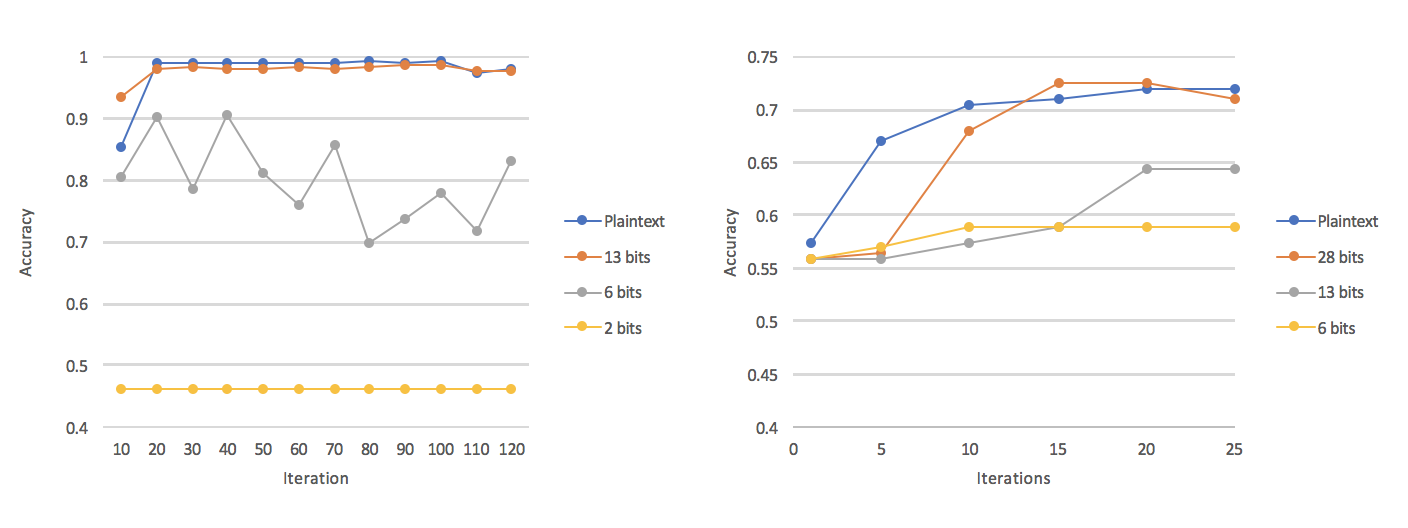
\includegraphics[scale=0.6]{mnistarcene.png}
  \caption{REPLACE THIS.}
  \label{fig:result4}
\end{figure}

\subsection{Neural Networks}

\section{Conclusion and Future Work}

Not sure what to write here..

\section{References}

\vc{will fix this later with bibtex}

[1] Privacy-Preserving Distributed Linear Regression on High-Dimensional Data

[2] SecureML

\end{document}